\documentclass[11pt,preprint]{elsarticle}

\usepackage{lmodern}
%%%% My spacing
\usepackage{setspace}
\setstretch{1.2}
\DeclareMathSizes{12}{14}{10}{10}

% Wrap around which gives all figures included the [H] command, or places it "here". This can be tedious to code in Rmarkdown.
\usepackage{float}
\let\origfigure\figure
\let\endorigfigure\endfigure
\renewenvironment{figure}[1][2] {
    \expandafter\origfigure\expandafter[H]
} {
    \endorigfigure
}

\let\origtable\table
\let\endorigtable\endtable
\renewenvironment{table}[1][2] {
    \expandafter\origtable\expandafter[H]
} {
    \endorigtable
}


\usepackage{ifxetex,ifluatex}
\usepackage{fixltx2e} % provides \textsubscript
\ifnum 0\ifxetex 1\fi\ifluatex 1\fi=0 % if pdftex
  \usepackage[T1]{fontenc}
  \usepackage[utf8]{inputenc}
\else % if luatex or xelatex
  \ifxetex
    \usepackage{mathspec}
    \usepackage{xltxtra,xunicode}
  \else
    \usepackage{fontspec}
  \fi
  \defaultfontfeatures{Mapping=tex-text,Scale=MatchLowercase}
  \newcommand{\euro}{€}
\fi

\usepackage{amssymb, amsmath, amsthm, amsfonts}

\def\bibsection{\section*{References}} %%% Make "References" appear before bibliography


\usepackage[numbers]{natbib}

\usepackage{longtable}
\usepackage[margin=2.3cm,bottom=2cm,top=2.5cm, includefoot]{geometry}
\usepackage{fancyhdr}
\usepackage[bottom, hang, flushmargin]{footmisc}
\usepackage{graphicx}
\numberwithin{equation}{section}
\numberwithin{figure}{section}
\numberwithin{table}{section}
\setlength{\parindent}{0cm}
\setlength{\parskip}{1.3ex plus 0.5ex minus 0.3ex}
\usepackage{textcomp}
\renewcommand{\headrulewidth}{0.2pt}
\renewcommand{\footrulewidth}{0.3pt}

\usepackage{array}
\newcolumntype{x}[1]{>{\centering\arraybackslash\hspace{0pt}}p{#1}}

%%%%  Remove the "preprint submitted to" part. Don't worry about this either, it just looks better without it:
\makeatletter
\def\ps@pprintTitle{%
  \let\@oddhead\@empty
  \let\@evenhead\@empty
  \let\@oddfoot\@empty
  \let\@evenfoot\@oddfoot
}
\makeatother

 \def\tightlist{} % This allows for subbullets!

\usepackage{hyperref}
\hypersetup{breaklinks=true,
            bookmarks=true,
            colorlinks=true,
            citecolor=blue,
            urlcolor=blue,
            linkcolor=blue,
            pdfborder={0 0 0}}


% The following packages allow huxtable to work:
\usepackage{siunitx}
\usepackage{multirow}
\usepackage{hhline}
\usepackage{calc}
\usepackage{tabularx}
\usepackage{booktabs}
\usepackage{caption}


\newenvironment{columns}[1][]{}{}

\newenvironment{column}[1]{\begin{minipage}{#1}\ignorespaces}{%
\end{minipage}
\ifhmode\unskip\fi
\aftergroup\useignorespacesandallpars}

\def\useignorespacesandallpars#1\ignorespaces\fi{%
#1\fi\ignorespacesandallpars}

\makeatletter
\def\ignorespacesandallpars{%
  \@ifnextchar\par
    {\expandafter\ignorespacesandallpars\@gobble}%
    {}%
}
\makeatother


% definitions for citeproc citations
\NewDocumentCommand\citeproctext{}{}
\NewDocumentCommand\citeproc{mm}{%
\href{\#cite.\detokenize{#1}}{#2}\nocite{#1}}

\makeatletter
% allow citations to break across lines
\let\@cite@ofmt\@firstofone
% avoid brackets around text for \cite:
\def\@biblabel#1{}
\def\@cite#1#2{{#1\if@tempswa , #2\fi}}
\makeatother
\newlength{\cslhangindent}
\setlength{\cslhangindent}{1.5em}
\newlength{\csllabelwidth}
\setlength{\csllabelwidth}{3em}
\newenvironment{CSLReferences}[2] % #1 hanging-indent, #2 entry-spacing
{\begin{list}{}{%
	\setlength{\itemindent}{0pt}
	\setlength{\leftmargin}{0pt}
	\setlength{\parsep}{0pt}
	% turn on hanging indent if param 1 is 1
	\ifodd #1
	\setlength{\leftmargin}{\cslhangindent}
	\setlength{\itemindent}{-1\cslhangindent}
	\fi
	% set entry spacing
	\setlength{\itemsep}{#2\baselineskip}}}
{\end{list}}

\usepackage{calc}
\newcommand{\CSLBlock}[1]{\hfill\break\parbox[t]{\linewidth}{\strut\ignorespaces#1\strut}}
\newcommand{\CSLLeftMargin}[1]{\parbox[t]{\csllabelwidth}{\strut#1\strut}}
\newcommand{\CSLRightInline}[1]{\parbox[t]{\linewidth - \csllabelwidth}{\strut#1\strut}}
\newcommand{\CSLIndent}[1]{\hspace{\cslhangindent}#1}


\urlstyle{same}  % don't use monospace font for urls
\setlength{\parindent}{0pt}
\setlength{\parskip}{6pt plus 2pt minus 1pt}
\setlength{\emergencystretch}{3em}  % prevent overfull lines
\setcounter{secnumdepth}{5}

%%% Use protect on footnotes to avoid problems with footnotes in titles
\let\rmarkdownfootnote\footnote%
\def\footnote{\protect\rmarkdownfootnote}
\IfFileExists{upquote.sty}{\usepackage{upquote}}{}

%%% Include extra packages specified by user

%%% Hard setting column skips for reports - this ensures greater consistency and control over the length settings in the document.
%% page layout
%% paragraphs
\setlength{\baselineskip}{12pt plus 0pt minus 0pt}
\setlength{\parskip}{12pt plus 0pt minus 0pt}
\setlength{\parindent}{0pt plus 0pt minus 0pt}
%% floats
\setlength{\floatsep}{12pt plus 0 pt minus 0pt}
\setlength{\textfloatsep}{20pt plus 0pt minus 0pt}
\setlength{\intextsep}{14pt plus 0pt minus 0pt}
\setlength{\dbltextfloatsep}{20pt plus 0pt minus 0pt}
\setlength{\dblfloatsep}{14pt plus 0pt minus 0pt}
%% maths
\setlength{\abovedisplayskip}{12pt plus 0pt minus 0pt}
\setlength{\belowdisplayskip}{12pt plus 0pt minus 0pt}
%% lists
\setlength{\topsep}{10pt plus 0pt minus 0pt}
\setlength{\partopsep}{3pt plus 0pt minus 0pt}
\setlength{\itemsep}{5pt plus 0pt minus 0pt}
\setlength{\labelsep}{8mm plus 0mm minus 0mm}
\setlength{\parsep}{\the\parskip}
\setlength{\listparindent}{\the\parindent}
%% verbatim
\setlength{\fboxsep}{5pt plus 0pt minus 0pt}



\begin{document}



\begin{frontmatter}  %

\title{Analysis of billionaires across the World}

% Set to FALSE if wanting to remove title (for submission)




\author[Add1]{Linda Dube}
\ead{23084103@sun.ac.za}





\address[Add1]{Stellenbosch University, Western Cape}


\begin{abstract}
\small{
This project developed a custom R function to efficiently load and
preprocess the billionaire dataset by utilizing column type metadata
from an Excel file, ensuring accurate data interpretation. Through
exploratory visualizations, key global trends in billionaire wealth
distribution and origins were identified across different decades. The
analysis employed diverse plots to test claims about self-made versus
inherited wealth patterns, providing data-driven insights into regional
and sectoral variations.
}
\end{abstract}

\vspace{1cm}


\begin{keyword}
\footnotesize{
Multivariate GARCH \sep Kalman Filter \sep Copula \\
\vspace{0.3cm}
}
\footnotesize{
\textit{JEL classification} L250 \sep L100
}
\end{keyword}



\vspace{0.5cm}

\end{frontmatter}

\setcounter{footnote}{0}



%________________________
% Header and Footers
%%%%%%%%%%%%%%%%%%%%%%%%%%%%%%%%%
\pagestyle{fancy}
\chead{}
\rhead{}
\lfoot{}
\rfoot{\footnotesize Page \thepage}
\lhead{}
%\rfoot{\footnotesize Page \thepage } % "e.g. Page 2"
\cfoot{}

%\setlength\headheight{30pt}
%%%%%%%%%%%%%%%%%%%%%%%%%%%%%%%%%
%________________________

\headsep 35pt % So that header does not go over title




\section{\texorpdfstring{Introduction
\label{Introduction}}{Introduction }}\label{introduction}

Forbes has commissioned this analysis to evaluate two central claims
about global billionaire wealth trends using data spanning three decades
(1990s--2010s). The first claim posits that the United States has seen a
rise in self-made billionaires with minimal generational wealth ties,
while other developed and emerging markets remain dominated by inherited
wealth. The second claim suggests that software has eclipsed consumer
services as the primary sector for new self-made billionaires, with this
shift linked to national GDP levels. By interrogating these assertions,
this report aims to uncover whether the data supports these patterns or
reveals more nuanced realities about wealth creation across regions and
industries. The findings will inform Forbes' ongoing efforts to refine
its billionaire database and provide evidence-based insights into global
economic mobility.

\section*{Data}\label{data}
\addcontentsline{toc}{section}{Data}

\begin{Shaded}
\begin{Highlighting}[]
\CommentTok{\# At the start of your Rmd or in a setup chunk:}
\ControlFlowTok{if}\NormalTok{ (}\SpecialCharTok{!}\FunctionTok{requireNamespace}\NormalTok{(}\StringTok{"readxl"}\NormalTok{, }\AttributeTok{quietly =} \ConstantTok{TRUE}\NormalTok{)) \{}
  \FunctionTok{install.packages}\NormalTok{(}\StringTok{"readxl"}\NormalTok{)}
\NormalTok{\}}
\FunctionTok{library}\NormalTok{(readxl)}
\end{Highlighting}
\end{Shaded}

\begin{verbatim}
## Warning: package 'readxl' was built under R version 4.4.3
\end{verbatim}

\begin{Shaded}
\begin{Highlighting}[]
\NormalTok{info }\OtherTok{\textless{}{-}} \FunctionTok{read\_excel}\NormalTok{(}\StringTok{"C:/Users/sukol/Documents/Masters frst semester/Data Science Exam/Data{-}Science{-}Exam/23084103\_Datascience\_Exam/Tex\_Ex/23084103\_Exam/Question 4/Tex\_Ex/23084103\_Billionaires/data/Billions/Info\_file.xlsx"}\NormalTok{)}

\FunctionTok{print}\NormalTok{(info)}
\end{Highlighting}
\end{Shaded}

\begin{verbatim}
## # A tibble: 19 x 4
##    Key                      `Column Type` Comment                `Example Value`
##    <chr>                    <chr>         <chr>                  <chr>          
##  1 name                     String        "The name of the bill~ "\"Bill Gates\~
##  2 rank                     Integer       "The rank of this bil~ "1"            
##  3 year                     Integer       "The year that data a~ "1996"         
##  4 company.founded          Integer       "The year that the co~ "1975"         
##  5 company.name             String        "The name of the comp~ "\"Microsoft\""
##  6 company.relationship     String        "The billionaires rel~ "\"founder\""  
##  7 company.sector           String        "The sector of the bu~ "\" Software\""
##  8 company.type             String        "The type of business~ "\"new\""      
##  9 demographics.age         Integer       "The current age of t~ "40"           
## 10 demographics.gender      String        "A string representin~ "\"male\""     
## 11 location.citizenship     String        "The name of the coun~ "\"United Stat~
## 12 location.country code    String        "the 3-letter country~ "\"USA\""      
## 13 location.gdp             Float         "The \"Gross Domestic~ "8100000000000"
## 14 location.region          String        "The region of the wo~ "\"North Ameri~
## 15 wealth.type              String        "The type of billiona~ "\"founder non~
## 16 wealth.worth in billions Float         "The number of billio~ "18.5"         
## 17 wealth.how.category      String        "A category represent~ "\"New Sectors~
## 18 wealth.how.industry      String        "The specific industr~ "\"Technology-~
## 19 wealth.how.inherited     String        "The way that this mo~ "\"not inherit~
\end{verbatim}

\begin{Shaded}
\begin{Highlighting}[]
\NormalTok{bespoke\_read\_function }\OtherTok{\textless{}{-}} \ControlFlowTok{function}\NormalTok{(csv\_path, info\_path) \{}
  \FunctionTok{library}\NormalTok{(readxl)}
  \FunctionTok{library}\NormalTok{(readr)}

  

  \CommentTok{\# Rename columns for clarity}
  \FunctionTok{colnames}\NormalTok{(info) }\OtherTok{\textless{}{-}} \FunctionTok{c}\NormalTok{(}\StringTok{"column\_name"}\NormalTok{, }\StringTok{"column\_type"}\NormalTok{)}

  \CommentTok{\# Map Excel column types to readr column specifications}
\NormalTok{  col\_types\_list }\OtherTok{\textless{}{-}} \FunctionTok{setNames}\NormalTok{(}
    \FunctionTok{lapply}\NormalTok{(info}\SpecialCharTok{$}\NormalTok{column\_type, }\ControlFlowTok{function}\NormalTok{(t) \{}
      \ControlFlowTok{switch}\NormalTok{(t,}
             \AttributeTok{String  =} \FunctionTok{col\_character}\NormalTok{(),}
             \AttributeTok{Integer =} \FunctionTok{col\_integer}\NormalTok{(),}
             \AttributeTok{Double  =} \FunctionTok{col\_double}\NormalTok{(),}
             \AttributeTok{Date    =} \FunctionTok{col\_date}\NormalTok{(}\AttributeTok{format =} \StringTok{""}\NormalTok{),}
             \FunctionTok{col\_skip}\NormalTok{()  }\CommentTok{\# fallback for unknown types}
\NormalTok{      )}
\NormalTok{    \}),}
\NormalTok{    info}\SpecialCharTok{$}\NormalTok{column\_name}
\NormalTok{  )}

  \CommentTok{\# Read the CSV file using the specified column types}
  \FunctionTok{read\_csv}\NormalTok{(csv\_path, }\AttributeTok{col\_types =} \FunctionTok{do.call}\NormalTok{(cols, col\_types\_list))}
\NormalTok{\}}


\NormalTok{billions }\OtherTok{\textless{}{-}} \FunctionTok{bespoke\_read\_function}\NormalTok{(}
  \AttributeTok{csv\_path =} \StringTok{"C:/Users/sukol/Documents/Masters frst semester/Data Science Exam/Data{-}Science{-}Exam/23084103\_Datascience\_Exam/Tex\_Ex/23084103\_Exam/Question 4/Tex\_Ex/23084103\_Billionaires/data/Billions/billionaires.csv"}\NormalTok{,}
  \AttributeTok{info\_path =} \StringTok{"C:/Users/sukol/Documents/Masters frst semester/Data Science Exam/Data{-}Science{-}Exam/23084103\_Datascience\_Exam/Tex\_Ex/23084103\_Exam/Question 4/Tex\_Ex/23084103\_Billionaires/data/Billions/Info\_file.xlsx"}
\NormalTok{)}
\end{Highlighting}
\end{Shaded}

\section{Data visualisation}\label{data-visualisation}

\subsection{Industry with more
billionaires}\label{industry-with-more-billionaires}

\begin{Shaded}
\begin{Highlighting}[]
\FunctionTok{library}\NormalTok{(ggplot2)}
\FunctionTok{library}\NormalTok{(dplyr)}
\end{Highlighting}
\end{Shaded}

\begin{verbatim}
## 
## Attaching package: 'dplyr'
\end{verbatim}

\begin{verbatim}
## The following objects are masked from 'package:stats':
## 
##     filter, lag
\end{verbatim}

\begin{verbatim}
## The following objects are masked from 'package:base':
## 
##     intersect, setdiff, setequal, union
\end{verbatim}

\begin{Shaded}
\begin{Highlighting}[]
\CommentTok{\# Count frequency of company sectors and select top 5}
\NormalTok{top\_sectors }\OtherTok{\textless{}{-}}\NormalTok{ billions }\SpecialCharTok{\%\textgreater{}\%}
  \FunctionTok{count}\NormalTok{(company.sector, }\AttributeTok{sort =} \ConstantTok{TRUE}\NormalTok{) }\SpecialCharTok{\%\textgreater{}\%}
  \FunctionTok{top\_n}\NormalTok{(}\DecValTok{5}\NormalTok{, n)}

\CommentTok{\# Plot bar chart of top 5 company sectors}
\FunctionTok{ggplot}\NormalTok{(top\_sectors, }\FunctionTok{aes}\NormalTok{(}\AttributeTok{x =} \FunctionTok{reorder}\NormalTok{(company.sector, n), }\AttributeTok{y =}\NormalTok{ n)) }\SpecialCharTok{+}
  \FunctionTok{geom\_bar}\NormalTok{(}\AttributeTok{stat =} \StringTok{"identity"}\NormalTok{, }\AttributeTok{fill =} \StringTok{"steelblue"}\NormalTok{) }\SpecialCharTok{+}
  \FunctionTok{coord\_flip}\NormalTok{() }\SpecialCharTok{+}  \CommentTok{\# flip coordinates to make it horizontal}
  \FunctionTok{labs}\NormalTok{(}
    \AttributeTok{title =} \StringTok{"Top 5 Company Sectors of Billionaires"}\NormalTok{,}
    \AttributeTok{x =} \StringTok{"Company Sector"}\NormalTok{,}
    \AttributeTok{y =} \StringTok{"Number of Billionaires"}
\NormalTok{  ) }\SpecialCharTok{+}
  \FunctionTok{theme\_minimal}\NormalTok{()}
\end{Highlighting}
\end{Shaded}

\begin{figure}

{\centering 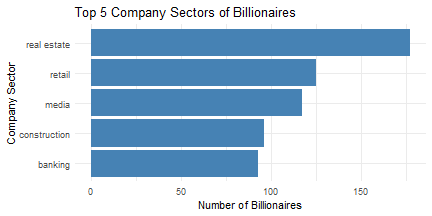
\includegraphics{23084103_Billionaires_files/figure-latex/Figure 1a-1} 

}

\caption{Caption Here \label{Figure1}}\label{fig:Figure 1a}
\end{figure}

The bar chart displays the top 5 company sectors where billionaires are
involved. Real estate leads significantly, having the highest number of
billionaires, followed by retail and media. Construction and banking
also feature prominently but with fewer billionaires. This suggests that
real estate is the most lucrative sector among billionaires in the data
set.

\subsection{Number of billionaires by
region}\label{number-of-billionaires-by-region}

\begin{Shaded}
\begin{Highlighting}[]
\FunctionTok{library}\NormalTok{(dplyr)}
\FunctionTok{library}\NormalTok{(ggplot2)}

\CommentTok{\# Group and count the number of billionaires per region}
\NormalTok{region\_counts }\OtherTok{\textless{}{-}}\NormalTok{ billions }\SpecialCharTok{\%\textgreater{}\%}
  \FunctionTok{group\_by}\NormalTok{(location.region) }\SpecialCharTok{\%\textgreater{}\%}
  \FunctionTok{summarise}\NormalTok{(}\AttributeTok{count =} \FunctionTok{n}\NormalTok{()) }\SpecialCharTok{\%\textgreater{}\%}
    \FunctionTok{arrange}\NormalTok{(}\FunctionTok{desc}\NormalTok{(count))}
  

\CommentTok{\# Bar plot}
\FunctionTok{ggplot}\NormalTok{(region\_counts, }\FunctionTok{aes}\NormalTok{(}\AttributeTok{x =} \FunctionTok{reorder}\NormalTok{(location.region, count), }\AttributeTok{y =}\NormalTok{ count)) }\SpecialCharTok{+}
  \FunctionTok{geom\_bar}\NormalTok{(}\AttributeTok{stat =} \StringTok{"identity"}\NormalTok{, }\AttributeTok{fill =} \StringTok{"skyblue"}\NormalTok{) }\SpecialCharTok{+}
  \FunctionTok{coord\_flip}\NormalTok{() }\SpecialCharTok{+}
  \FunctionTok{labs}\NormalTok{(}
    \AttributeTok{title =} \StringTok{"Number of Billionaires by Region"}\NormalTok{,}
    \AttributeTok{x =} \StringTok{"Region"}\NormalTok{,}
    \AttributeTok{y =} \StringTok{"Number of Billionaires"}
\NormalTok{  ) }\SpecialCharTok{+}
  \FunctionTok{theme\_minimal}\NormalTok{()}
\end{Highlighting}
\end{Shaded}

\begin{figure}

{\centering 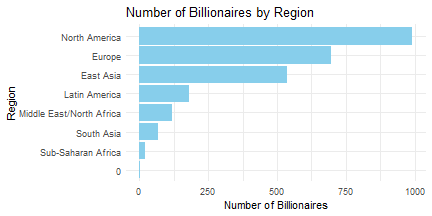
\includegraphics{23084103_Billionaires_files/figure-latex/Figure 1b-1} 

}

\caption{Caption Here \label{Figure1}}\label{fig:Figure 1b}
\end{figure}

This bar plot displays the number of billionaires across different
global regions. North America leads by a wide margin, hosting nearly
1,000 billionaires, highlighting its strong economic concentration.
Europe and East Asia follow, each with several hundred billionaires,
reflecting their established and emerging markets. Other regions like
Latin America, Middle East/North Africa, and South Asia show
significantly fewer billionaires, while Sub-Saharan Africa has the
lowest count, suggesting disparities in wealth accumulation and economic
opportunity across regions.

\section{Analysis}\label{analysis}

\begin{Shaded}
\begin{Highlighting}[]
  \CommentTok{\# This is just a random plot to show you a plot. This is done if the getwd() does not point to your Template\textquotesingle{}s directory.}
  

 \FunctionTok{library}\NormalTok{(ggplot2)}
\FunctionTok{library}\NormalTok{(dplyr)}

\CommentTok{\# Filter for U.S. billionaires only}
\NormalTok{us\_billionaires }\OtherTok{\textless{}{-}}\NormalTok{ billions }\SpecialCharTok{\%\textgreater{}\%}
  \FunctionTok{filter}\NormalTok{(location.citizenship }\SpecialCharTok{==} \StringTok{"United States"}\NormalTok{)}

\CommentTok{\# Group by decade and inheritance status}
\NormalTok{us\_line\_data }\OtherTok{\textless{}{-}}\NormalTok{ us\_billionaires }\SpecialCharTok{\%\textgreater{}\%}
  \FunctionTok{mutate}\NormalTok{(}\AttributeTok{decade =} \FunctionTok{floor}\NormalTok{(year }\SpecialCharTok{/} \DecValTok{10}\NormalTok{) }\SpecialCharTok{*} \DecValTok{10}\NormalTok{) }\SpecialCharTok{\%\textgreater{}\%}
  \FunctionTok{group\_by}\NormalTok{(decade, wealth.how.inherited) }\SpecialCharTok{\%\textgreater{}\%}
  \FunctionTok{summarise}\NormalTok{(}\AttributeTok{count =} \FunctionTok{n}\NormalTok{(), }\AttributeTok{.groups =} \StringTok{"drop"}\NormalTok{)}

\CommentTok{\# Plot the line graph}
\FunctionTok{ggplot}\NormalTok{(us\_line\_data, }\FunctionTok{aes}\NormalTok{(}\AttributeTok{x =}\NormalTok{ decade, }\AttributeTok{y =}\NormalTok{ count, }\AttributeTok{color =}\NormalTok{ wealth.how.inherited)) }\SpecialCharTok{+}
  \FunctionTok{geom\_line}\NormalTok{(}\AttributeTok{size =} \FloatTok{1.2}\NormalTok{) }\SpecialCharTok{+}
  \FunctionTok{geom\_point}\NormalTok{(}\AttributeTok{size =} \DecValTok{4}\NormalTok{) }\SpecialCharTok{+}
  \FunctionTok{scale\_x\_continuous}\NormalTok{(}\AttributeTok{breaks =} \FunctionTok{seq}\NormalTok{(}\FunctionTok{min}\NormalTok{(us\_line\_data}\SpecialCharTok{$}\NormalTok{decade), }\FunctionTok{max}\NormalTok{(us\_line\_data}\SpecialCharTok{$}\NormalTok{decade), }\DecValTok{10}\NormalTok{),}
                     \AttributeTok{labels =} \ControlFlowTok{function}\NormalTok{(x) }\FunctionTok{paste0}\NormalTok{(x, }\StringTok{"s"}\NormalTok{)) }\SpecialCharTok{+}
  \FunctionTok{labs}\NormalTok{(}
    \AttributeTok{title =} \StringTok{"Trends in Wealth Accumulation Among U.S. Billionaires"}\NormalTok{,}
    \AttributeTok{x =} \StringTok{"Decade"}\NormalTok{,}
    \AttributeTok{y =} \StringTok{"Number of Billionaires"}\NormalTok{,}
    \AttributeTok{color =} \StringTok{"Inheritance Status"}
\NormalTok{  ) }\SpecialCharTok{+}
  \FunctionTok{theme\_minimal}\NormalTok{(}\AttributeTok{base\_size =} \DecValTok{14}\NormalTok{) }\SpecialCharTok{+}
  \FunctionTok{theme}\NormalTok{(}
    \AttributeTok{plot.title =} \FunctionTok{element\_text}\NormalTok{(}\AttributeTok{hjust =} \FloatTok{0.5}\NormalTok{, }\AttributeTok{size =} \DecValTok{10}\NormalTok{),}
    \AttributeTok{legend.title =} \FunctionTok{element\_text}\NormalTok{(}\AttributeTok{size =} \DecValTok{10}\NormalTok{),}
    \AttributeTok{legend.text =} \FunctionTok{element\_text}\NormalTok{(}\AttributeTok{size =} \DecValTok{10}\NormalTok{),}
    \AttributeTok{legend.key.size =} \FunctionTok{unit}\NormalTok{(}\FloatTok{0.4}\NormalTok{, }\StringTok{"cm"}\NormalTok{)}
\NormalTok{  )}
\end{Highlighting}
\end{Shaded}

\begin{figure}

{\centering 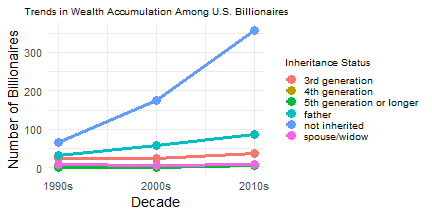
\includegraphics{23084103_Billionaires_files/figure-latex/Figure 2a-1} 

}

\caption{Caption Here \label{Figure1}}\label{fig:Figure 2a}
\end{figure}

The graph shows a steady dominance of ``not inherited'' wealth among US
billionaires across the decades. Starting in the 1990s, billionaires
without generational wealth were already the largest group, but this
number increased sharply after 2000, indicating a rise in self-made
billionaires. The second most common inheritance path is wealth from
fathers, while other categories like ``3rd generation'',
``spouse/widow'', and ``5th generation or longer'' remain consistently
low and relatively unchanged over time.The data supports the first part
of the claim: ``In the US, you saw an increasing number of new
billionaires emerge that had little to no familial ties to generational
wealth.'' Indeed, the number of self-made billionaires in the US ---
those who did not inherit their wealth --- has grown significantly,
especially after the early 2000s. This suggests an increasing trend of
entrepreneurial success and new wealth creation.

\subsection{Other countries}\label{other-countries}

\begin{Shaded}
\begin{Highlighting}[]
\FunctionTok{library}\NormalTok{(ggplot2)}
\FunctionTok{library}\NormalTok{(dplyr)}

\CommentTok{\# Filter for U.S. billionaires only}
\NormalTok{Mexico\_billionaires }\OtherTok{\textless{}{-}}\NormalTok{ billions }\SpecialCharTok{\%\textgreater{}\%}
  \FunctionTok{filter}\NormalTok{(location.citizenship }\SpecialCharTok{==} \StringTok{"Mexico"}\NormalTok{)}

\CommentTok{\# Group by decade and inheritance status}
\NormalTok{Mexico\_line\_data }\OtherTok{\textless{}{-}}\NormalTok{ Mexico\_billionaires }\SpecialCharTok{\%\textgreater{}\%}
  \FunctionTok{mutate}\NormalTok{(}\AttributeTok{decade =} \FunctionTok{floor}\NormalTok{(year }\SpecialCharTok{/} \DecValTok{10}\NormalTok{) }\SpecialCharTok{*} \DecValTok{10}\NormalTok{) }\SpecialCharTok{\%\textgreater{}\%}
  \FunctionTok{group\_by}\NormalTok{(decade, wealth.how.inherited) }\SpecialCharTok{\%\textgreater{}\%}
  \FunctionTok{summarise}\NormalTok{(}\AttributeTok{count =} \FunctionTok{n}\NormalTok{(), }\AttributeTok{.groups =} \StringTok{"drop"}\NormalTok{)}

\CommentTok{\# Plot the line graph}
\FunctionTok{ggplot}\NormalTok{(Mexico\_line\_data, }\FunctionTok{aes}\NormalTok{(}\AttributeTok{x =}\NormalTok{ decade, }\AttributeTok{y =}\NormalTok{ count, }\AttributeTok{color =}\NormalTok{ wealth.how.inherited)) }\SpecialCharTok{+}
  \FunctionTok{geom\_line}\NormalTok{(}\AttributeTok{size =} \FloatTok{1.2}\NormalTok{) }\SpecialCharTok{+}
  \FunctionTok{geom\_point}\NormalTok{(}\AttributeTok{size =} \DecValTok{4}\NormalTok{) }\SpecialCharTok{+}
  \FunctionTok{scale\_x\_continuous}\NormalTok{(}\AttributeTok{breaks =} \FunctionTok{seq}\NormalTok{(}\FunctionTok{min}\NormalTok{(us\_line\_data}\SpecialCharTok{$}\NormalTok{decade), }\FunctionTok{max}\NormalTok{(us\_line\_data}\SpecialCharTok{$}\NormalTok{decade), }\DecValTok{10}\NormalTok{),}
                     \AttributeTok{labels =} \ControlFlowTok{function}\NormalTok{(x) }\FunctionTok{paste0}\NormalTok{(x, }\StringTok{"s"}\NormalTok{)) }\SpecialCharTok{+}
  \FunctionTok{labs}\NormalTok{(}
    \AttributeTok{title =} \StringTok{"Trends in Wealth Accumulation Among Mexico Billionaires"}\NormalTok{,}
    \AttributeTok{x =} \StringTok{"Decade"}\NormalTok{,}
    \AttributeTok{y =} \StringTok{"Number of Billionaires"}\NormalTok{,}
    \AttributeTok{color =} \StringTok{"Inheritance Status"}
\NormalTok{  ) }\SpecialCharTok{+}
  \FunctionTok{theme\_minimal}\NormalTok{(}\AttributeTok{base\_size =} \DecValTok{14}\NormalTok{) }\SpecialCharTok{+}
  \FunctionTok{theme}\NormalTok{(}
    \AttributeTok{plot.title =} \FunctionTok{element\_text}\NormalTok{(}\AttributeTok{hjust =} \FloatTok{0.5}\NormalTok{, }\AttributeTok{size =} \DecValTok{10}\NormalTok{),}
    \AttributeTok{legend.title =} \FunctionTok{element\_text}\NormalTok{(}\AttributeTok{size =} \DecValTok{10}\NormalTok{),}
    \AttributeTok{legend.text =} \FunctionTok{element\_text}\NormalTok{(}\AttributeTok{size =} \DecValTok{10}\NormalTok{),}
    \AttributeTok{legend.key.size =} \FunctionTok{unit}\NormalTok{(}\FloatTok{0.4}\NormalTok{, }\StringTok{"cm"}\NormalTok{)}
\NormalTok{  )}
\end{Highlighting}
\end{Shaded}

\begin{figure}

{\centering 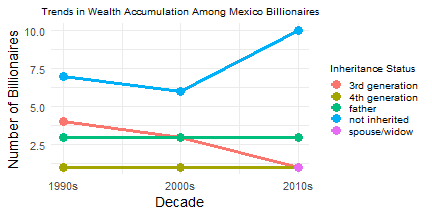
\includegraphics{23084103_Billionaires_files/figure-latex/Figure 2b-1} 

}

\caption{Caption Here \label{Figure1}}\label{fig:Figure 2b}
\end{figure}

\begin{Shaded}
\begin{Highlighting}[]
\FunctionTok{library}\NormalTok{(ggplot2)}
\FunctionTok{library}\NormalTok{(dplyr)}

\CommentTok{\# Filter for U.S. billionaires only}
\NormalTok{saudi\_billionaires }\OtherTok{\textless{}{-}}\NormalTok{ billions }\SpecialCharTok{\%\textgreater{}\%}
  \FunctionTok{filter}\NormalTok{(location.citizenship }\SpecialCharTok{==} \StringTok{"Saudi Arabia"}\NormalTok{)}

\CommentTok{\# Group by decade and inheritance status}
\NormalTok{Saudi\_line\_data }\OtherTok{\textless{}{-}}\NormalTok{ saudi\_billionaires }\SpecialCharTok{\%\textgreater{}\%}
  \FunctionTok{mutate}\NormalTok{(}\AttributeTok{decade =} \FunctionTok{floor}\NormalTok{(year }\SpecialCharTok{/} \DecValTok{10}\NormalTok{) }\SpecialCharTok{*} \DecValTok{10}\NormalTok{) }\SpecialCharTok{\%\textgreater{}\%}
  \FunctionTok{group\_by}\NormalTok{(decade, wealth.how.inherited) }\SpecialCharTok{\%\textgreater{}\%}
  \FunctionTok{summarise}\NormalTok{(}\AttributeTok{count =} \FunctionTok{n}\NormalTok{(), }\AttributeTok{.groups =} \StringTok{"drop"}\NormalTok{)}

\CommentTok{\# Plot the line graph}
\FunctionTok{ggplot}\NormalTok{(Saudi\_line\_data, }\FunctionTok{aes}\NormalTok{(}\AttributeTok{x =}\NormalTok{ decade, }\AttributeTok{y =}\NormalTok{ count, }\AttributeTok{color =}\NormalTok{ wealth.how.inherited)) }\SpecialCharTok{+}
  \FunctionTok{geom\_line}\NormalTok{(}\AttributeTok{size =} \FloatTok{1.2}\NormalTok{) }\SpecialCharTok{+}
  \FunctionTok{geom\_point}\NormalTok{(}\AttributeTok{size =} \DecValTok{4}\NormalTok{) }\SpecialCharTok{+}
  \FunctionTok{scale\_x\_continuous}\NormalTok{(}\AttributeTok{breaks =} \FunctionTok{seq}\NormalTok{(}\FunctionTok{min}\NormalTok{(us\_line\_data}\SpecialCharTok{$}\NormalTok{decade), }\FunctionTok{max}\NormalTok{(us\_line\_data}\SpecialCharTok{$}\NormalTok{decade), }\DecValTok{10}\NormalTok{),}
                     \AttributeTok{labels =} \ControlFlowTok{function}\NormalTok{(x) }\FunctionTok{paste0}\NormalTok{(x, }\StringTok{"s"}\NormalTok{)) }\SpecialCharTok{+}
  \FunctionTok{labs}\NormalTok{(}
    \AttributeTok{title =} \StringTok{"Trends in Wealth Accumulation Among Saudi Arabia\textquotesingle{}s Billionaires"}\NormalTok{,}
    \AttributeTok{x =} \StringTok{"Decade"}\NormalTok{,}
    \AttributeTok{y =} \StringTok{"Number of Billionaires"}\NormalTok{,}
    \AttributeTok{color =} \StringTok{"Inheritance Status"}
\NormalTok{  ) }\SpecialCharTok{+}
  \FunctionTok{theme\_minimal}\NormalTok{(}\AttributeTok{base\_size =} \DecValTok{14}\NormalTok{) }\SpecialCharTok{+}
  \FunctionTok{theme}\NormalTok{(}
    \AttributeTok{plot.title =} \FunctionTok{element\_text}\NormalTok{(}\AttributeTok{hjust =} \FloatTok{0.5}\NormalTok{, }\AttributeTok{size =} \DecValTok{10}\NormalTok{),}
    \AttributeTok{legend.title =} \FunctionTok{element\_text}\NormalTok{(}\AttributeTok{size =} \DecValTok{10}\NormalTok{),}
    \AttributeTok{legend.text =} \FunctionTok{element\_text}\NormalTok{(}\AttributeTok{size =} \DecValTok{10}\NormalTok{),}
    \AttributeTok{legend.key.size =} \FunctionTok{unit}\NormalTok{(}\FloatTok{0.4}\NormalTok{, }\StringTok{"cm"}\NormalTok{)}
\NormalTok{  )}
\end{Highlighting}
\end{Shaded}

\begin{figure}

{\centering 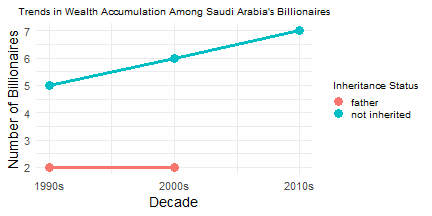
\includegraphics{23084103_Billionaires_files/figure-latex/Figure 2c-1} 

}

\caption{Caption Here \label{Figure1}}\label{fig:Figure 2c}
\end{figure}

\begin{Shaded}
\begin{Highlighting}[]
\FunctionTok{library}\NormalTok{(ggplot2)}

\FunctionTok{library}\NormalTok{(dplyr)}

\CommentTok{\# Filter for U.S. billionaires only}
\NormalTok{SA\_billionaires }\OtherTok{\textless{}{-}}\NormalTok{ billions }\SpecialCharTok{\%\textgreater{}\%}
  \FunctionTok{filter}\NormalTok{(location.citizenship }\SpecialCharTok{==} \StringTok{"South Africa"}\NormalTok{)}

\CommentTok{\# Group by decade and inheritance status}
\NormalTok{SA\_line\_data }\OtherTok{\textless{}{-}}\NormalTok{ SA\_billionaires }\SpecialCharTok{\%\textgreater{}\%}
  \FunctionTok{mutate}\NormalTok{(}\AttributeTok{decade =} \FunctionTok{floor}\NormalTok{(year }\SpecialCharTok{/} \DecValTok{10}\NormalTok{) }\SpecialCharTok{*} \DecValTok{10}\NormalTok{) }\SpecialCharTok{\%\textgreater{}\%}
  \FunctionTok{group\_by}\NormalTok{(decade, wealth.how.inherited) }\SpecialCharTok{\%\textgreater{}\%}
  \FunctionTok{summarise}\NormalTok{(}\AttributeTok{count =} \FunctionTok{n}\NormalTok{(), }\AttributeTok{.groups =} \StringTok{"drop"}\NormalTok{)}

\CommentTok{\# Plot the line graph}
\FunctionTok{ggplot}\NormalTok{(SA\_line\_data, }\FunctionTok{aes}\NormalTok{(}\AttributeTok{x =}\NormalTok{ decade, }\AttributeTok{y =}\NormalTok{ count, }\AttributeTok{color =}\NormalTok{ wealth.how.inherited)) }\SpecialCharTok{+}
  \FunctionTok{geom\_line}\NormalTok{(}\AttributeTok{size =} \FloatTok{1.2}\NormalTok{) }\SpecialCharTok{+}
  \FunctionTok{geom\_point}\NormalTok{(}\AttributeTok{size =} \DecValTok{4}\NormalTok{) }\SpecialCharTok{+}
  \FunctionTok{scale\_x\_continuous}\NormalTok{(}\AttributeTok{breaks =} \FunctionTok{seq}\NormalTok{(}\FunctionTok{min}\NormalTok{(us\_line\_data}\SpecialCharTok{$}\NormalTok{decade), }\FunctionTok{max}\NormalTok{(us\_line\_data}\SpecialCharTok{$}\NormalTok{decade), }\DecValTok{10}\NormalTok{),}
                     \AttributeTok{labels =} \ControlFlowTok{function}\NormalTok{(x) }\FunctionTok{paste0}\NormalTok{(x, }\StringTok{"s"}\NormalTok{)) }\SpecialCharTok{+}
  \FunctionTok{labs}\NormalTok{(}
    \AttributeTok{title =} \StringTok{"Trends in Wealth Accumulation Among SA Billionaires"}\NormalTok{,}
    \AttributeTok{x =} \StringTok{"Decade"}\NormalTok{,}
    \AttributeTok{y =} \StringTok{"Number of Billionaires"}\NormalTok{,}
    \AttributeTok{color =} \StringTok{"Inheritance Status"}
\NormalTok{  ) }\SpecialCharTok{+}
  \FunctionTok{theme\_minimal}\NormalTok{(}\AttributeTok{base\_size =} \DecValTok{14}\NormalTok{) }\SpecialCharTok{+}
  \FunctionTok{theme}\NormalTok{(}
    \AttributeTok{plot.title =} \FunctionTok{element\_text}\NormalTok{(}\AttributeTok{hjust =} \FloatTok{0.5}\NormalTok{, }\AttributeTok{size =} \DecValTok{10}\NormalTok{),}
    \AttributeTok{legend.title =} \FunctionTok{element\_text}\NormalTok{(}\AttributeTok{size =} \DecValTok{10}\NormalTok{),}
    \AttributeTok{legend.text =} \FunctionTok{element\_text}\NormalTok{(}\AttributeTok{size =} \DecValTok{10}\NormalTok{),}
    \AttributeTok{legend.key.size =} \FunctionTok{unit}\NormalTok{(}\FloatTok{0.4}\NormalTok{, }\StringTok{"cm"}\NormalTok{)}
\NormalTok{  )}
\end{Highlighting}
\end{Shaded}

\begin{figure}

{\centering 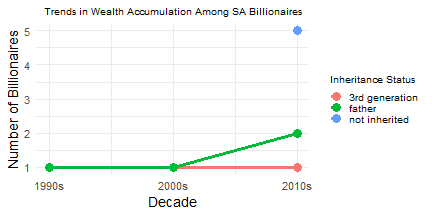
\includegraphics{23084103_Billionaires_files/figure-latex/Figure 2d-1} 

}

\caption{Caption Here \label{Figure1}}\label{fig:Figure 2d}
\end{figure}

The plots results above challenge the latter part of the claim that
emerging and developed markets tend to house mostly inherited wealth. In
Mexico, the pattern closely mirrors the U.S., with a dominant presence
of self-made billionaires and shifting inheritance trends over time,
showing strong entrepreneurial emergence. In contrast, countries like
Saudi Arabia and South Africa show different dynamics, mainly due to a
smaller billionaire population, making it harder to generalize trends.
Despite lower representation, not all wealth in these nations stems from
inheritance, suggesting nuanced paths to wealth. Therefore, the claim
oversimplifies the diversity of wealth accumulation across global
markets.

\newpage

\section{Conclusion}\label{conclusion}

The analysis substantiates the claim that the U.S. has experienced a
significant increase in self-made billionaires, with data showing a
clear decline in reliance on inherited wealth over time. However, it
challenges the broader generalization about other markets, as countries
like Mexico demonstrate similar entrepreneurial trends, while others
(e.g., Saudi Arabia) exhibit context-specific wealth accumulation
patterns. Sector-wise, real estate---not software---remains the dominant
industry for billionaire wealth, though technology-driven economies show
growing influence in newer wealth creation. These findings underscore
the need for Forbes to adopt a more nuanced framework for assessing
global wealth dynamics, one that accounts for regional variations and
evolving sectoral impacts. The data reaffirms the rise of self-made
wealth in the U.S. but cautions against oversimplifying the diverse
pathways to billionaire status worldwide

\bibliography{Tex/ref}





\end{document}
